\subsubsection{Llargada del formulari}

\paragraph{}
Aquesta funcionalitat, pot arribar a presentar un formulari relativament llarg, si considerem tots els camps, en teoria disponibles, de cara a la cerca de persones. Per aquest motiu, s'han dissenyat un parell de funcionalitats que pretenen facilitar la comprensió i utilització del formulari de cerca.

La primera d'elles, consisteix en què els formularis referents a la persona cercada i els seus relatius més propers, poden ser plegats i desplegats, mitjançant un clic en la capçalera del bloc.

Per tal d'indicar que es pot interactuar amb aquestes capçaleres, s'ha afegit el signe `-' o `+', a l'esquerra del títol i una icona que també reflecteix l'estat actual a la dreta. A la vegada, un text en cursiva, explica la funcionalitat en la mateixa barra i en passar el ratolí per sobre de la capçalera, aquesta canvia de color i transforma la icona del ratolí, en una mà d'interacció.

La segona funcionalitat, té l'objectiu de facilitar la iniciació de la cerca. En moltes circumstàncies, els usuaris només voldran emplenar detalls bàsics de la persona principal a cercar i no pas les dels seus relatius. Per aquest motiu, només el formulari de cerca de la persona principal es troba desplegat d'entrada. Aquest fet, implica que el botó de cerca pot quedar molt allunyat de l'inici del formulari i per tant, pot resultar confús pels usuaris com iniciar la cerca.

Per evitar aquesta confusió, un cop se superen 780 píxels de la posició inicial del formulari i fins que s'arriba a la posició original del botó de cerca, una barra fixa apareix al final de la pàgina, amb el botó de cerca i se sobreposa al contingut de la pàgina web. D'aquesta forma, el botó de cerca queda accessible en tot moment pels usuaris, sense la necessitat d'arribar al final del formulari.

La figura~\ref{fig:interactiveFormBloc} mostra els dos estats possibles de les capçaleres dels blocs del for\-mu\-la\-ri i la barra que se sobreposa al contingut de la pàgina web i que apareix al final de la pantalla, amb el botó de cerca, quan es compleixen les condicions necessàries.

\begin{figure}[h]
    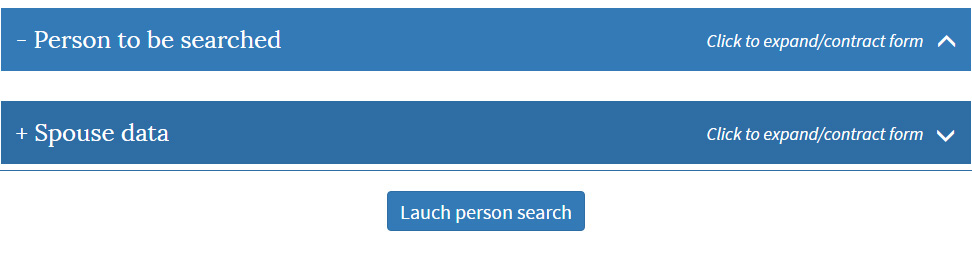
\includegraphics[width=\linewidth]{11/02_searchPersons/03_formBars}
    \centering
    \caption{Blocs de formulari interactius i sobreposició del botó de cerca}\label{fig:interactiveFormBloc}
\end{figure}

L'efecte de la barra sobre impressionada amb el botó de cerca, s'aconsegueix mitjançant jQuery i el canvi de classes CSS, en els elements HTML que contenen la barra de cerca. El jQuery s'encarrega d'espiar la posició de l'usuari, cada cop que es desplaça verticalment per la pàgina web i les diferents classes CSS, fixen o alliberen la posició del contenidor de la barra de cerca, segons aquesta posició.

A continuació, mostrem la classe CSS que converteix la barra de cerca, en una barra de posició fixa al final de la pàgina web. Les principals propietats que ho fan possible són: \emph{position:fixed} i \emph{bottom: 0px}.

\begin{lstlisting}[style=rawOwn,caption={Classe CSS per sobre impressionar el botó de cerca}]
.detached-bottom {
    position: fixed;
    bottom: 0px;
    height: 80px;
    width: 100%;
    margin-top: 0px;
    border-top: 1px solid #2e6da4;
    z-index: 9999;
    background-color: #fff;
    -webkit-transition: all 0.2s linear;
    -moz-transition: all 0.2s linear;
    -o-transition: all 0.2s linear;
    transition: all 0.2s linear;
}
\end{lstlisting}
